\chapter{Concept}
\label{ch:concept}
The main aim of the task is to setup the drone to work in the environment of Robot Operating System (ROS) for the purpose of custom ORBSLAM3 package development which estimates Camera Pose and Keyframe trajectory in any given coordinate system. Orbslam3 or Orbslam in general computes and detects key points on the image frame using ORB features and estimates camera pose of the current frame in real-time. Camera pose data consists of the position of the camera center in the orbslam coordinate system and orientation of the camera with respect to the orbslam coordinate system. These results helps in 3D reconstruction or scene reconstruction. The camera poses and trajectory can be scaled to any coordinate system of our choice namely ENU or ECEF for a global view. \\

Previously, every other experiment on the topic of Visual SLAM or VI-SLAM were processed offline using recorded data. This approach takes a step ahead to run the SLAM systems while the drone is flying and get the live camera poses and keyframe trajectory. The usage of ROS bolsters our approach by providing real-time data publishing-subscribing platform on par for an online processing scheme. Even though Orbslam3 native library supports Visual SLAM and VI-SLAM without ROS environment, developing a custom package using ROS and SLAM systems provided by the native library creates a flexible support for the usage of APIs. \\

Initial goal was to run the Visual SLAM and VI-SLAM on the drone and test the ORBSLAM3's out-of-box functionalities and to understand the resources which paves way to the planning for the development course. Moreover, to achieve this, it needs prerequisites such as setting up the drone's on-board computer (Manifold 2) by installing SDK and ROS SDK for our needs. Moving on, as sections of this chapter, we shall discuss and explain different prerequisite tasks that were carried out to support the main goal.

\section{Initial Architecture}
\label{sec:concept:archi}
Architecture, as shown in the Fig Fig \ref{fig:architecture}, of any major task plays an important role to have a basic understanding of the system development and to list out sub sections in the development phase of a package. The architecture described below is architecture of the ROS package named as \texttt{vid\_orbslam3}. The main node in the package subscribes to image topic in our case named as  \texttt{/dji\_osdk\_ros/main\_camera\_images} published by the drone's on-board computer for the purpose of Visual SLAM and subscribes to both image topic and IMU topic i.e \texttt{/dji\_osdk\_ros/imu} for the purpose of VI-SLAM. Therefore, these two ROS topics published by bringing up the drone is used as inputs to our custom orbslam3 node. \texttt{vid\_orbslam3} node make use of orbslam3 library classes and methods to setup a SLAM mechanism in the ROS environment. Additional features such as saving the camera intrinsic parameters, Hamilton Quaternion Multiplier method and saving the Keyframe trajectory data into a file are developed into the \texttt{vid\_orbslam3} package. \\

We finally expect two fruitful outputs namely Camera Poses and Keyframe trajectory. These two results are to be published as Keyframe Graph as a custom posearray topic. This is the basic architecture planned for the initial phase of the development. After looking at the results, other parts of the architecture are to be added and facilitated. 

\begin{figure}
    \centering
    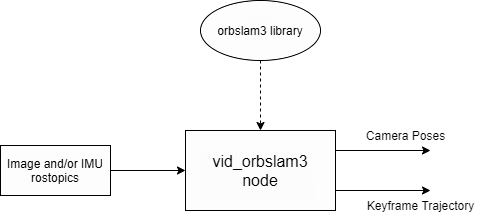
\includegraphics[height=5cm, width=9cm]{Images/archi.png}
    \caption{Architecture}
    \label{fig:architecture}
\end{figure}

\section{Setting up manifold 2 on-board computer}
\label{sec:concept:settingupmanifold}
The on-board computer supported by the DJI Matrice 210 series drone is Manifold 2. As discussed in technical background chapter, Manifold 2 runs on Ubuntu 16.04. Therefore, this computer runs as similar to as any other ubuntu system. This eases out the installation process of tools and libraries for the development. To access the data out of the drone peripherals and sensors for the purpose of processing, a SDK is needed. DJI developer community provides DJI onboard SDK \cite{DJI_OSDK} and DJI Onboard ROS SDK \cite{DJI_OSDK_ROS}. \\

At first, DJI Onboard SDK was installed onto the Manifold 2 using DJI's official documentation. Tests such as gimbal control, camera selection were performed using example code provided by the SDK package. This SDK installation is prerequisite for installing Onboard ROS SDK. As the task needs ROS environment development, ROS Kinetic Kame distribution was chosen to be installed on the Manifold 2 as Ubuntu 16.04 supports only Kinetic Kame. Following the official ROS documentation, ROS was installed and a separate work space for the development was created. It was also noted that, OpenCV 3.3.1-dev version was installed along with ROS. The OpenCV version installed on the system might affect or impact on the development of the \texttt{vid\_orbslam3} package using native orbslam3 library. \\

Further, Onboard ROS SDK was installed using standard ROS package installation into the ROS work space. The following commands were used compile the Onboard ROS SDK into the ROS work space:

\begin{lstlisting}[language=bash, basicstyle=\small]
$ cd catkin_ws/src
$ git clone https://github.com/dji-sdk/Onboard-SDK-ROS.git
$ cd ..
$ catkin_make 
\end{lstlisting}

Once the compilation ends, the onboard SDK for ROS is ready for usage. The ROS SDK comes with a launch file under launch folder which should be used to bring up the drone for ROS functionalities. It helps us launch the vehicle node that brings up the drone to ROS environment and publishes the peripheral and sensor data as ROS topics. These topics can be used by other nodes to their extent by subscription. This launch file is named as \texttt{dji\_vehicle\_node.launch} and contains few arguments related to user details. These details are generated when the drone is registered on the official portal for development purposes. A UserConfig.txt file is generated when the DJI Onboard SDK was installed. Fill in information available on UserConfig text file as it is into the argument fields inside the launch file. Without this step, drone cannot be made functional with the launch file. The vehicle node can be launched using the following commands:

\begin{lstlisting}[language=bash, basicstyle=\small]
$ roscore
$ roslaunch dji_osdk_ros dji_vehicle_node.launch
\end{lstlisting} 

ROS topics are published under the tag \texttt{/dji\_osdk\_ros/t\_name} and topics include main camera images, FPV images, left and right stereo images, IMU, GPS, gimbal angle and other useful topics.

\subsection*{Initiate Main Camera Images publishing}
\label{subsec:settingupmanifold:inititecamera}
With DJI ROS SDK, the camera topics are available as ROS topics once the vehicle node is brought up. But the data is not available until the camera service is called manually using rosservice call. This is done to reduce the overhead on the vehicle node to omit the camera topics which are not needed. Camera service call is available for all the cameras namely main camera, FPV camera and stereo cameras. Therefore, a shell script was written to automate the bringing up of the drone and select the required camera topics to publish.
Since, the task was mainly using the main camera, \texttt{/setup\_camera\_stream} service was available and rosservice was called with suitable inputs to trigger the publish.

\section{Installing ORBSLAM3 Library}
\label{sec:concept:orbslam3lib}
As discussed earlier, ORBSLAM3 library provides classes and methods to perform Visual SLAM, VI-SLAM and multi-map SLAM. Based on the official documentation, ORBSLAM3 library was tested on Ubuntu 16.04 and 18.04. This library requires C++11 compiler, Pangolin tool for visualization purposes, atleast OpenCV 3.0 and Eigen library 3.1.0 version or higher. ROS installation is optional for compiling the ORBSLAM3, but as per the task we have installed ROS as well. ORBSLAM3 was compiled following the instructions given in the official documentation. \\

Initially it was compiled and tested on a local computer having Ubuntu 18.04 and other required dependencies before it was compiled on the Manifold 2. Using the example code and EuRoC data set \cite{Burri25012016} (V1\_02\_medium.bag), ORBSLAM3 Monocular Visual SLAM and VI-SLAM were tested for better understanding of the library offered. Further, the same procedure was followed to compile the library on the Manifold 2. 

\vspace{1cm}
In the next chapter, we shall discuss on the implementation of the task. This task is divided into two parts. In the first part, the development of the vid\_orbslam3 package for Visual SLAM and VI-SLAM are explained, discussion on IMU sensor calibration and computing body-camera transformation matrix, discussion on failure of VI-SLAM on our setup and observations made on other SLAM systems such as Vins-Mono \cite{qin2017vins} and open\_vins \cite{Geneva2020ICRA}.
